\chapter{Results}
\label{chap:results}


Spatially and spectrally resolved line emission was detected for CO (3-2), HCO$^{+}$ (4-3), HCN (4-3), and CS (7-6) across around 50 channels of width 0.42 km s$^{-1}$. Here are presented line-emission statistics, as well as moment maps, channel maps, and a discussion on the role of cloud contamination in the data.


\bigskip

\section{Cloud Contamination}
% Ex footnote: \texttt{K2Phot}\footnote{\href{https://github.com/vincentvaneylen/k2photometry}{https://github.com/vincentvaneylen/k2photometry}} \citep{vaneylen2016}

Cloud contamination occurs when emission from gas clouds along the observation's line of sight is detected. This is typically not a significant issue for observations of proplyds in low-mass star forming regions (SFRs), but thanks to the Orion Nebula's significantly higher gas density, cloud contamination presents significant problems in these data, particularly in the CO line, thanks to its low critical density and relatively high abundance in the background clouds. Thanks to higher critical densities and lower abundances, cloud contamination is less significant, but still present, in the other lines. It is crucial to manage and minimize these effects before modeling so that cloud emission does not confuse the modeling algorithms.

\bigskip

Luckily, there exist ways to minimize the effects of cloud contamination. Here we take advantage of the fact that the structure of these contaminating clouds tends to be very large in scale (relative to a proplyd's length scales) and that, in observations made with interferometers like ALMA, one may control not only the smallest angular scales observed but also the largest angular scales observed. This is a feature unique to interferometers; while the designer of an optical telescope may increase their lens diameter to resolve smaller angular scales (analogous, in an interferometer, to increasing their maximum baseline distance), they may not control the largest angular scales resolved, since glass is a continuous substance whose "shortest diameter" cannot be changed (which would be analogous to varying the shortest baseline of an interferometer). Using these two features, we may exclude a selection of the shortest baselines used in our data, effectively shrinking the largest angular scales and, consequently, significantly reducing the effects of the cloud emission. While this process slightly reduces the total recovered flux from the disks and our ability to characterize their large-scale structures, it is a necessary process in order to avoid including cloud emission from the cloud in the process of fitting the disk emission. By evaluating mean and RMS noise for an off-source region of the field while varying the minimum baseline used, we found that excluding baselines less than 110 k$\lambda$, 80 k$\lambda$, and 60  k$\lambda$ for HCO$^{+}$, HCN, and CO, respectively, yielded optimum results. Since emission from the CS line already has a very low SNR and a higher critical density, excluding baselines did not improve the observations. The effects of different cuts is presented in the figure below.

\bigskip
\bigskip

% Calculations for this are made in scratch_02.py but maybe should be in scratch_03 now.
\begin{tabular}{l*{6}{c}r}
  \hline\hline \\

  \shortstack{Molecular \\ Line} & \shortstack{Baselines \\ Included} & \shortstack{Max Angular Scale \\ (")} & \shortstack{Integrated Line Flux [Disk A, Disk B]\\ (Jy km s$^{-1}$)} \\
  \hline
  CS (7-6)         & All                            & 8."5 & [837, 139] $\pm$ 0.07 \\
  CO (3-2)         & All                            & 8."4 & [837, 139] $\pm$ 0.07 \\
  CO (3-2)         & \textgreater 60 k$\lambda$     & 3."4 & [837, 139] $\pm$ 0.07 \\
  HCN (4-3)        & All                            & 8."2 & [837, 139] $\pm$ 0.07 \\
  HCN (4-3)        & \textgreater 80 k$\lambda$     & 2."6 & [837, 139] $\pm$ 0.07 \\
  HCO$^{+}$ (4-3)  & All                            & 8."2 & [837, 139] $\pm$ 0.07 \\
  HCO$^{+}$ (4-3)  & \textgreater 110 k$\lambda$    & 1."9 & [837, 139] $\pm$ 0.07 \\
  \hline
  \label{baseline_cutting_table}
\end{tabular}
\caption{Table 1: Integrated Flux Measurements}
\bigskip
\bigskip


% NOISE PROFILES
\begin{figure}
\centering
\begin{minipage}{.48\textwidth}
  \centering
  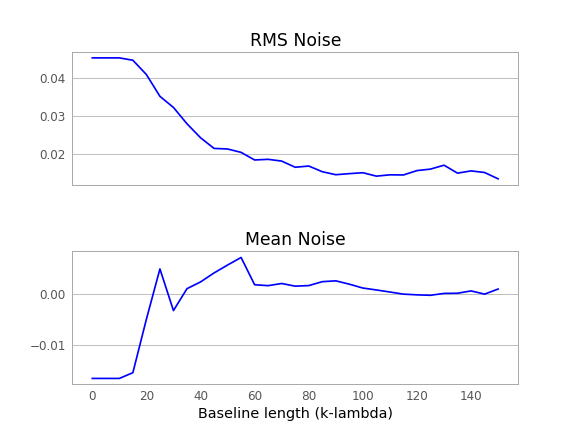
\includegraphics[width=\linewidth]{hco-imnoise_hco10000.png}
  \captionof{figure}{HCO Noise profiles}
  \label{fig:test1}
\end{minipage}%
\begin{minipage}{.48\textwidth}
  \centering
  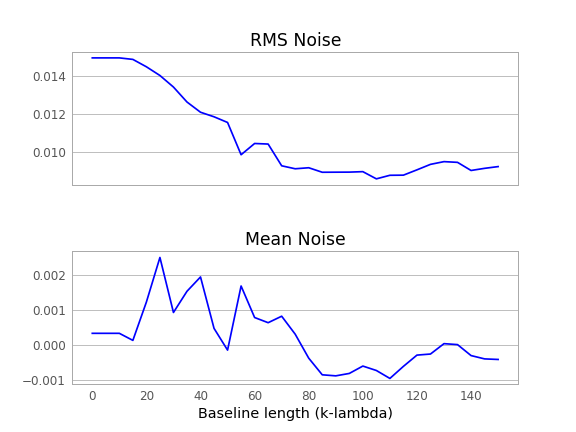
\includegraphics[width=\linewidth]{hcn-imnoise_hcn10000.png}
  \captionof{figure}{HCN Noise profiles}
  \label{fig:test2}
\end{minipage}
\end{figure}


\section{Line Data}

Moment maps offer us ways to flatten the three-dimensional data-cube (in $v, \alpha, \delta$) into two dimensions. Moment 0 maps integrate flux along the velocity axis as a function of position, providing insight into structures of emission intensity in the disk's morphology, while moment 1 maps, a velocity-weighted intensity integration across position, describe a source's velocity gradients. Figures \ref{fig:CO_m0} and \ref{fig:CO_m1} show zeroth- and first-moment maps, respectively, of the CO line emission, with and without a 60 k$\lambda$ baseline cut made (left and right, respectively).

% MOMENT MAPS
\begin{figure}
\centering
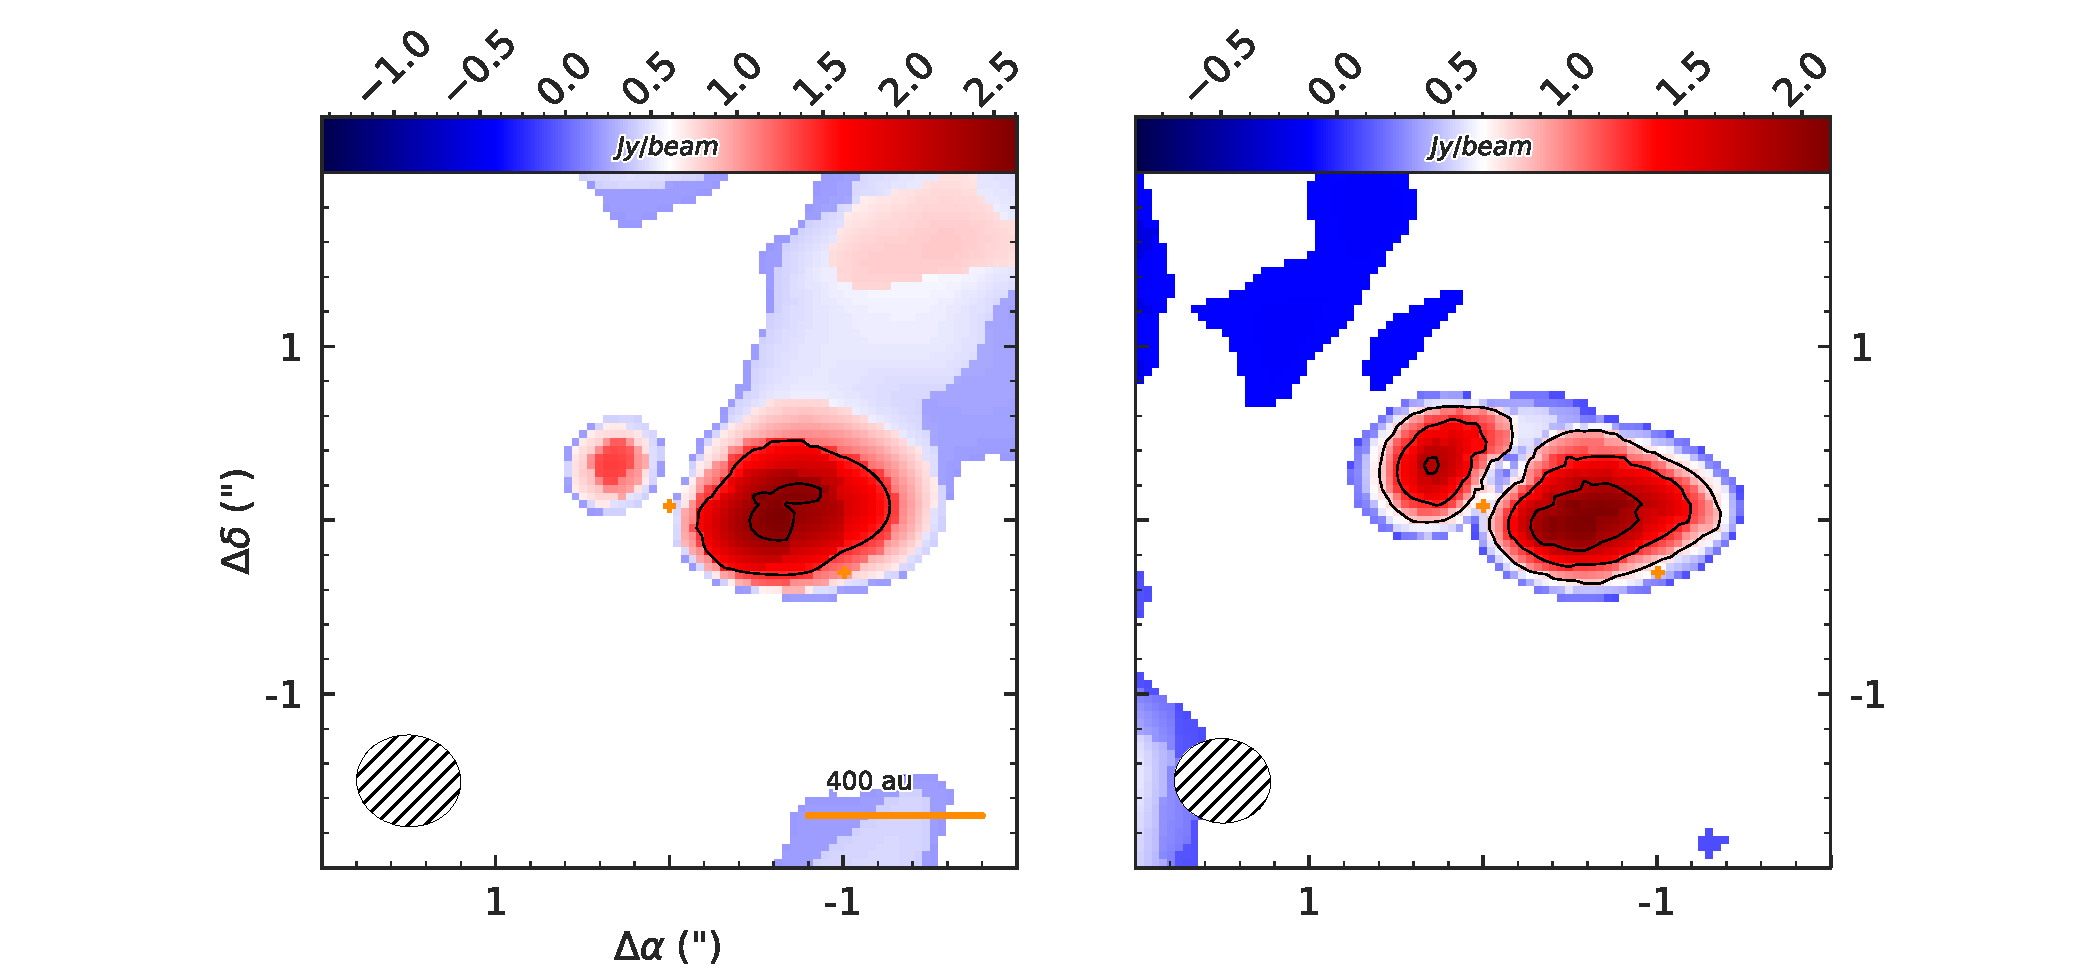
\includegraphics[width=\linewidth]{m0-map_co-co.pdf}[h!]
  \captionof{figure}{Zeroth moment map of CO emission, with and without a cut of all baseline's below 60 k$\lambda$ (left and right, respectively). Colors correspond to velocity-integrated intensity, while contours represent $\pm$3, 5, 7...15-$\sigma$ transitions where 1$\sigma$ is 0.257 Jy beam$^{-1}$ km s$^{-1}$. Negative contours are dashed. The beam is shown in the bottom left corner, with a diameter of 0."5 which corresponds to 200 AU at 389 parsec.}
  \label{fig:CO_m0}
  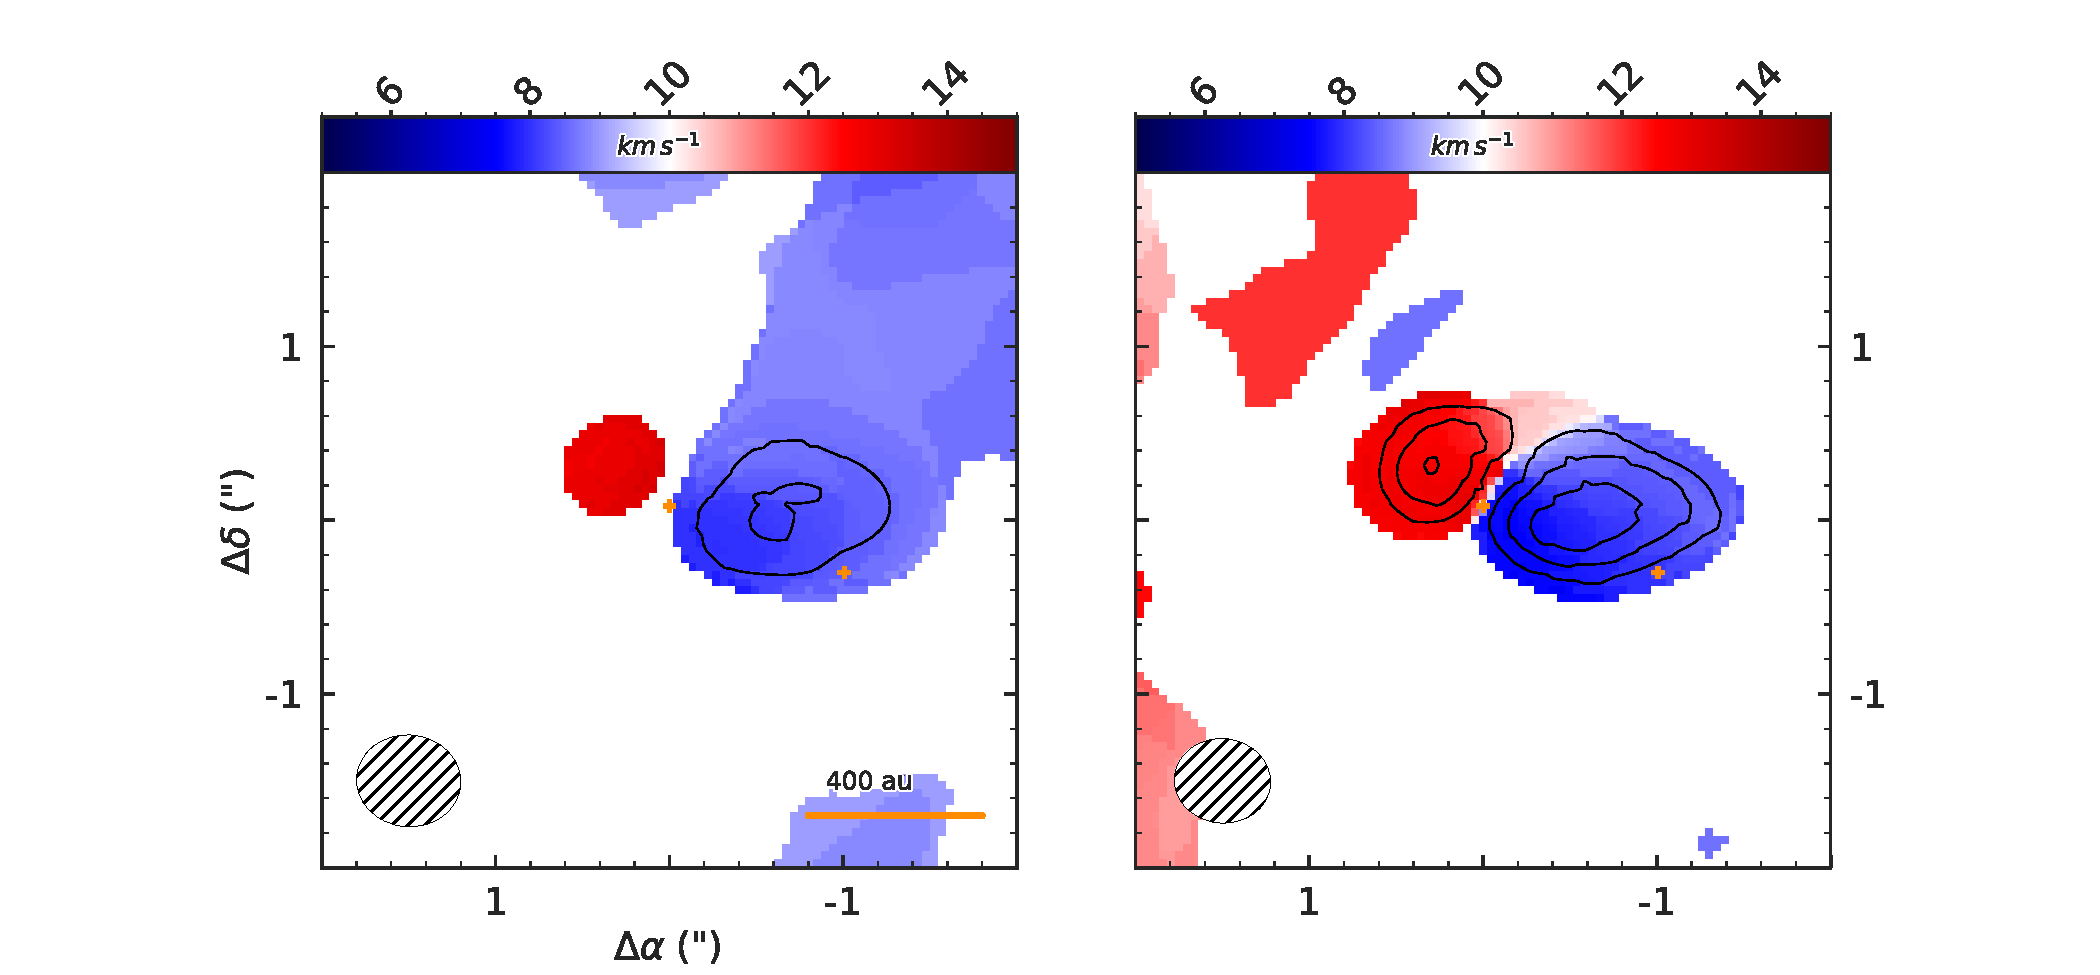
\includegraphics[width=\linewidth]{m1-map_co-co.pdf}
  \captionof{figure}{First moment map of CO emission, with and without a cut of all baseline's below 60 k$\lambda$ (left and right, respectively). Colors correspond to intensity-weighted LSRK velocity, while contours represent $\pm$3, 5, 7,..., 15-$\sigma$ transitions where 1$\sigma$ is 0.257 Jy beam$^{-1}$ km s$^{-1}$}
  \label{fig:CO_m1}
\end{figure}



Integrated line flux was measured using the Miriad task \texttt{cgcurs} to spatially integrate flux in a zeroth moment map over the region enclosed by the 3$\sigma$ contour. Unfortunately, results are several orders of magnitude off, so something seems to be wrong.

Elliptical Gaussian fits were attempted using both the CASA task \texttt{uvmodelfit} and the Miriad task \texttt{uvfit} before the author woke up enough to realize that something smarter would have to be done to separate the two disks. I think I did this over the summer, so it's just a matter of going back through old notes and remembering what the task was (I think it was an interactive CASA tool.) Additionally, I used the Gaussian fit tool in \texttt{imview} to go for rough fits. The reported extent of Disk A's major axis in the HCO+ line corresponds to an outer diameter of 500 AU; it was getting confused trying to fit for disk B. More work to be done here.

% uvfit vis=data/hco/hco-short110.vis object=gaussian



\iffalse
Tables 2 and 3 present the velocity-integrated line fluxes and the best-fit parameters for a simple elliptical Gaussian fit to the visibilities for each disk, respectively. Integrated line flux was measured using the MIRIAD task \texttt{cgcurs} to integrate the intensity in the zeroth-moment map throughout the region enclosed by the 3 $\sigma$ contour level. Uncertainties in the integrated line flux do not include the 10\% absolute flux calibration uncertainty inherent in the ALMA observations caused by uncertainties int he models of solar system objects used as flux callibrators. Elliptical Gaussian fits of the visibilities were performed using the MIRIAD task \texttt{uvfit}.
\fi

\bigskip

Assuming optically thin emission and Local Thermodynamic Equilibrium (LTE), the line-emitting gas mass, M$_{\text{gas}}$ is given by:

\begin{align}
  M_{\text{gas}}= \frac{4 \pi}{h \nu_0} \frac{F m d^2}{A_{ul} X_u},
  \label{M_gas}
\end{align}

where $F$ is the integrated line flux, $m$ is the mass of the emitting gas molecule, $d$ is the distance to the source, $h$ is the Planck constant, $\nu_0$ is the molecular line's rest frequency, $A_{ul}$ is the Einstein coefficient for the ($u - l$) transition, and

\begin{align}
  X_u = \frac{N_u}{N_{\text{tot}}} = (2 J_u + 1) \frac{\exp [-B_0 J_u (J_u + 1) h c/kT_{\text{ex}}]}{kT_{\text{ex}}/hc B_0}.
  \label{X_u}
\end{align}

In \ref{X_u}, $\frac{N_u}{N_{\text{tot}}}$ is the ratio of the number of molecules in the upper state to the total number of molecules; $J_u$ is the quantum number of the upper level; $B_0$ is the rotation constant in units of wavenumber; $h$ and $c$ are the Planck constant and speed of light, respectively; and $T_{\text{ex}}$ is the excitation temperature. Values for $A_{ul}$ and $B_0$ were taken from molecular data drawn from \citet{Schoeier_et_al_2005}. Since \ref{M_gas} is the mass of the observed gas species, it must be scaled by the it's relative abundance (fit for in Section 4) to obtain a total mass (\textit{I'm not totally clear on this}). From this, we find a total mass of $0.x \pm 0.y M_{\odot}$.



\begin{figure}
\centering
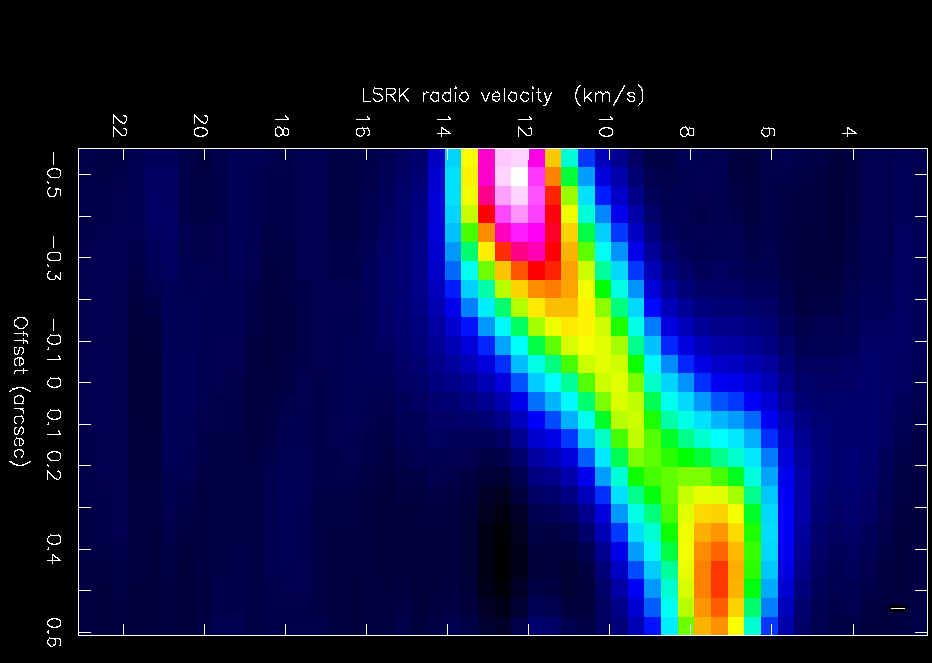
\includegraphics[width=\linewidth]{hco_pv_rough}[h!]
  \captionof{figure}{A bad PV diagram. I've figured out roughly how to do it but am still working out some kinks.}
  \label{fig:pv_diag}
\end{figure}

A Position-Velocity (PV) diagram is presented in \ref{fig:pv_diag}. The diagram shows the velocity distribution of of emission along a slice along the major axis of one of the disks. Since this is kinda garbage right now, there's not too much to say, but at least it's going somewhere.





I'm not sure if there's much to be gained from having channel maps in this section. Sam used them here a little to demonstrate an improvement in cloud contamination from cutting baselines, but I feel like moment maps do that pretty well.

\begin{figure}
\centering
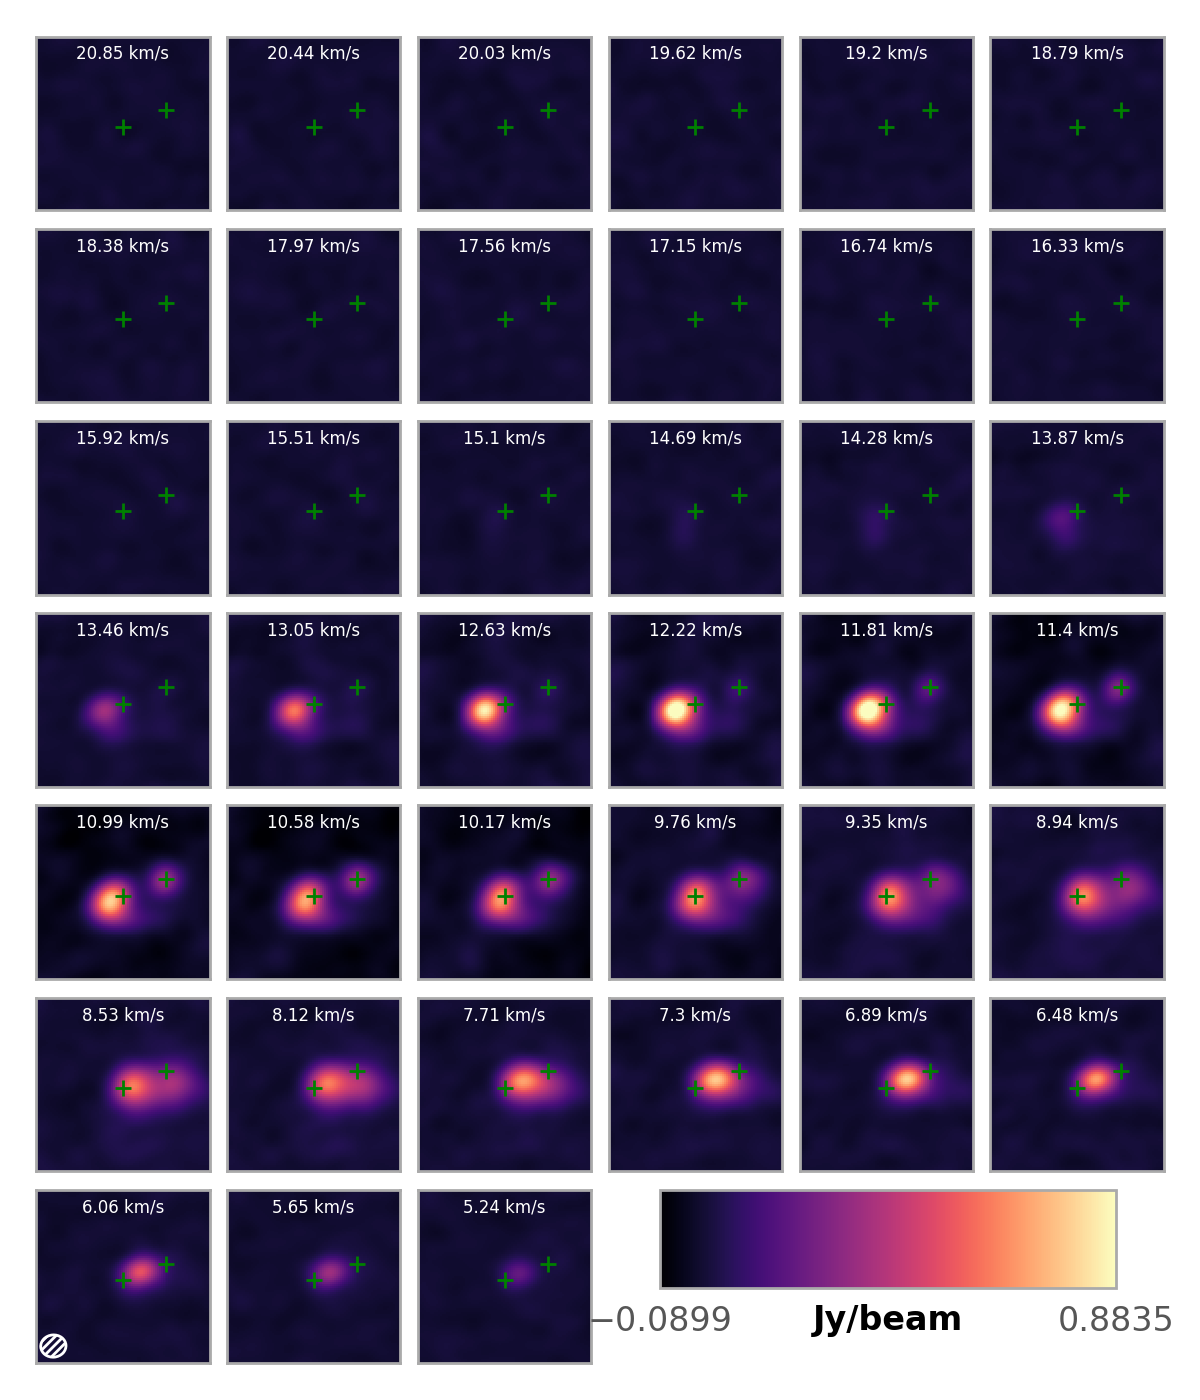
\includegraphics[width=\linewidth]{hco_image.png}[h!]
  \captionof{figure}{A rough channel map of the HCO+ data. This will get made into a better plotter later. I think it's good to have some channel maps in this section?}
  \label{fig:CO_m0}
\end{figure}











\iffalse
Things to get:
* Rewrite this whole thing.
* Integrated Flux Measurements
* Find max width of disks for each line by 3-sigma contour

* use uvfit for elliptical guassian vis fits.

\fi

\iffalse
\begin{figure}
\centering
\begin{minipage}{.5\textwidth}
  \centering
  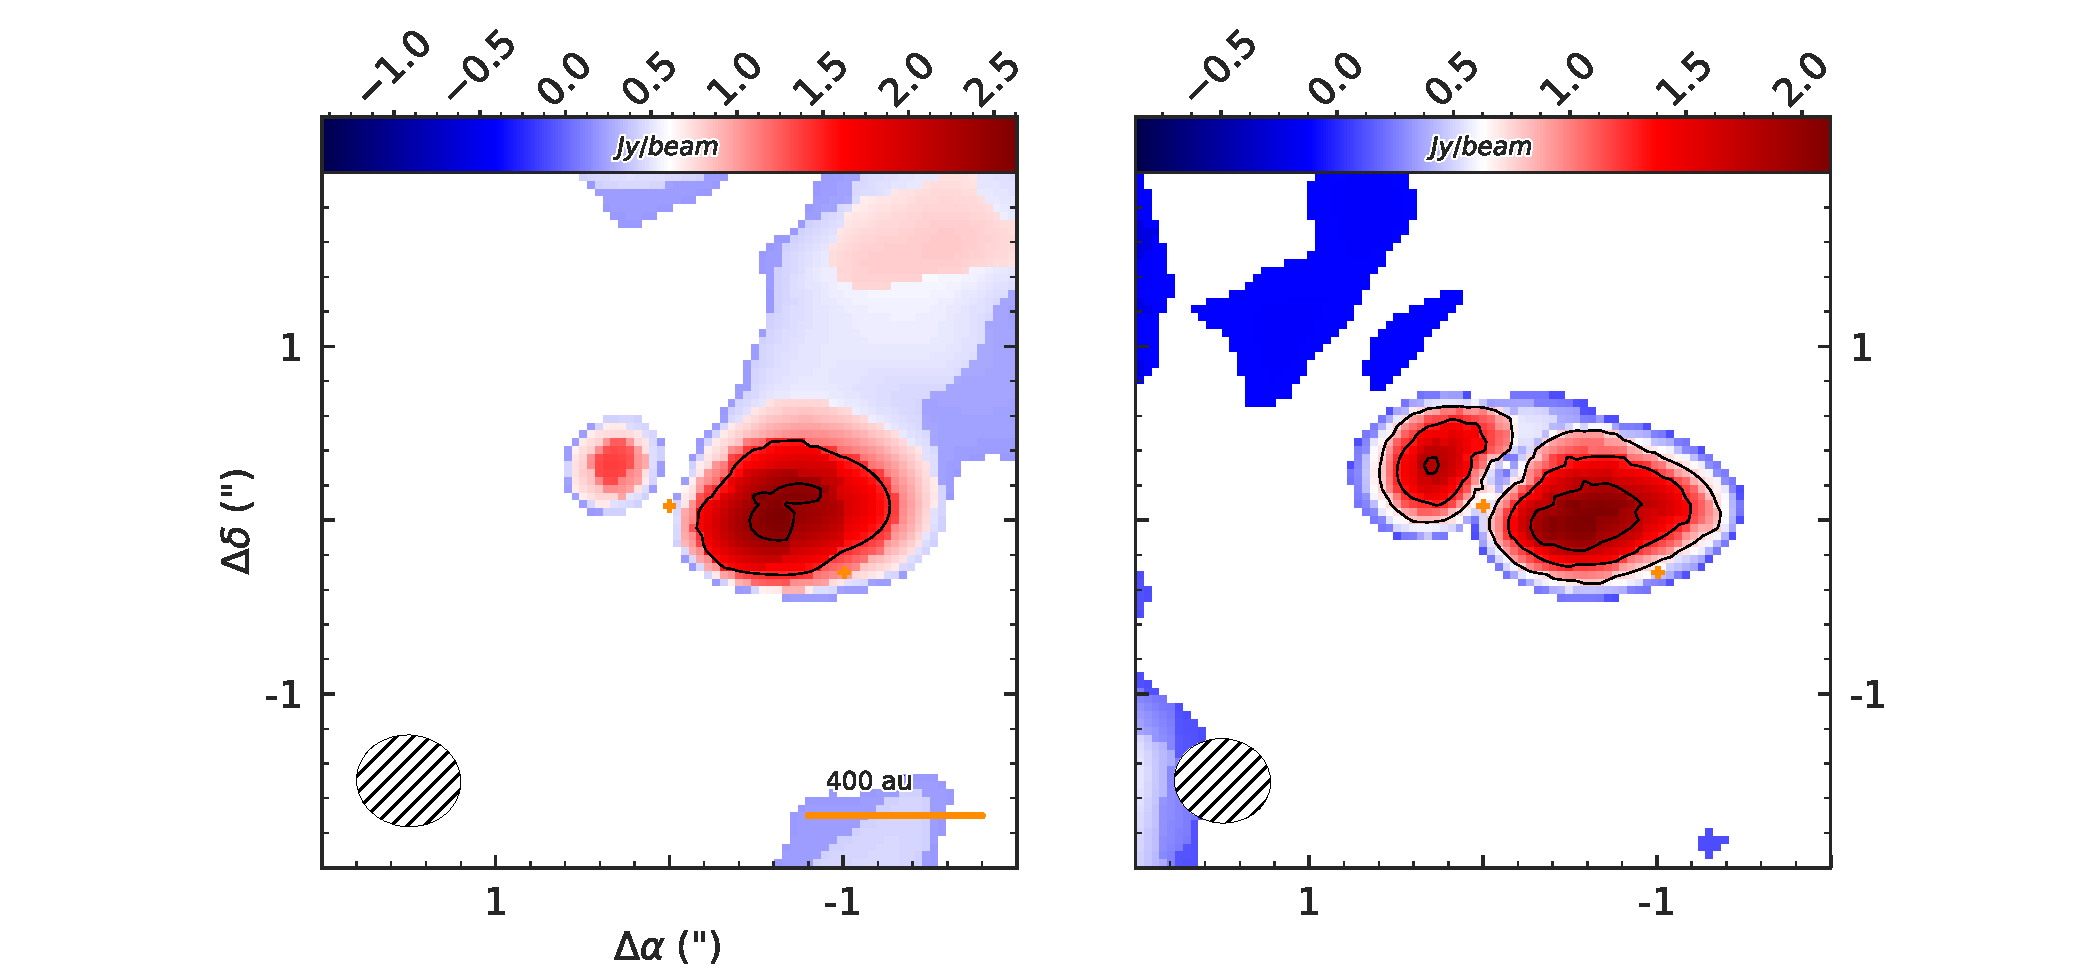
\includegraphics[width=.99\linewidth]{m0-map_co-co.pdf}
  \captionof{figure}{First moment map of HCO+, with and without (below and above, respectively) baseline cuts.}
  \label{fig:test1}
\end{minipage}%
\begin{minipage}{.5\textwidth}
  \centering
  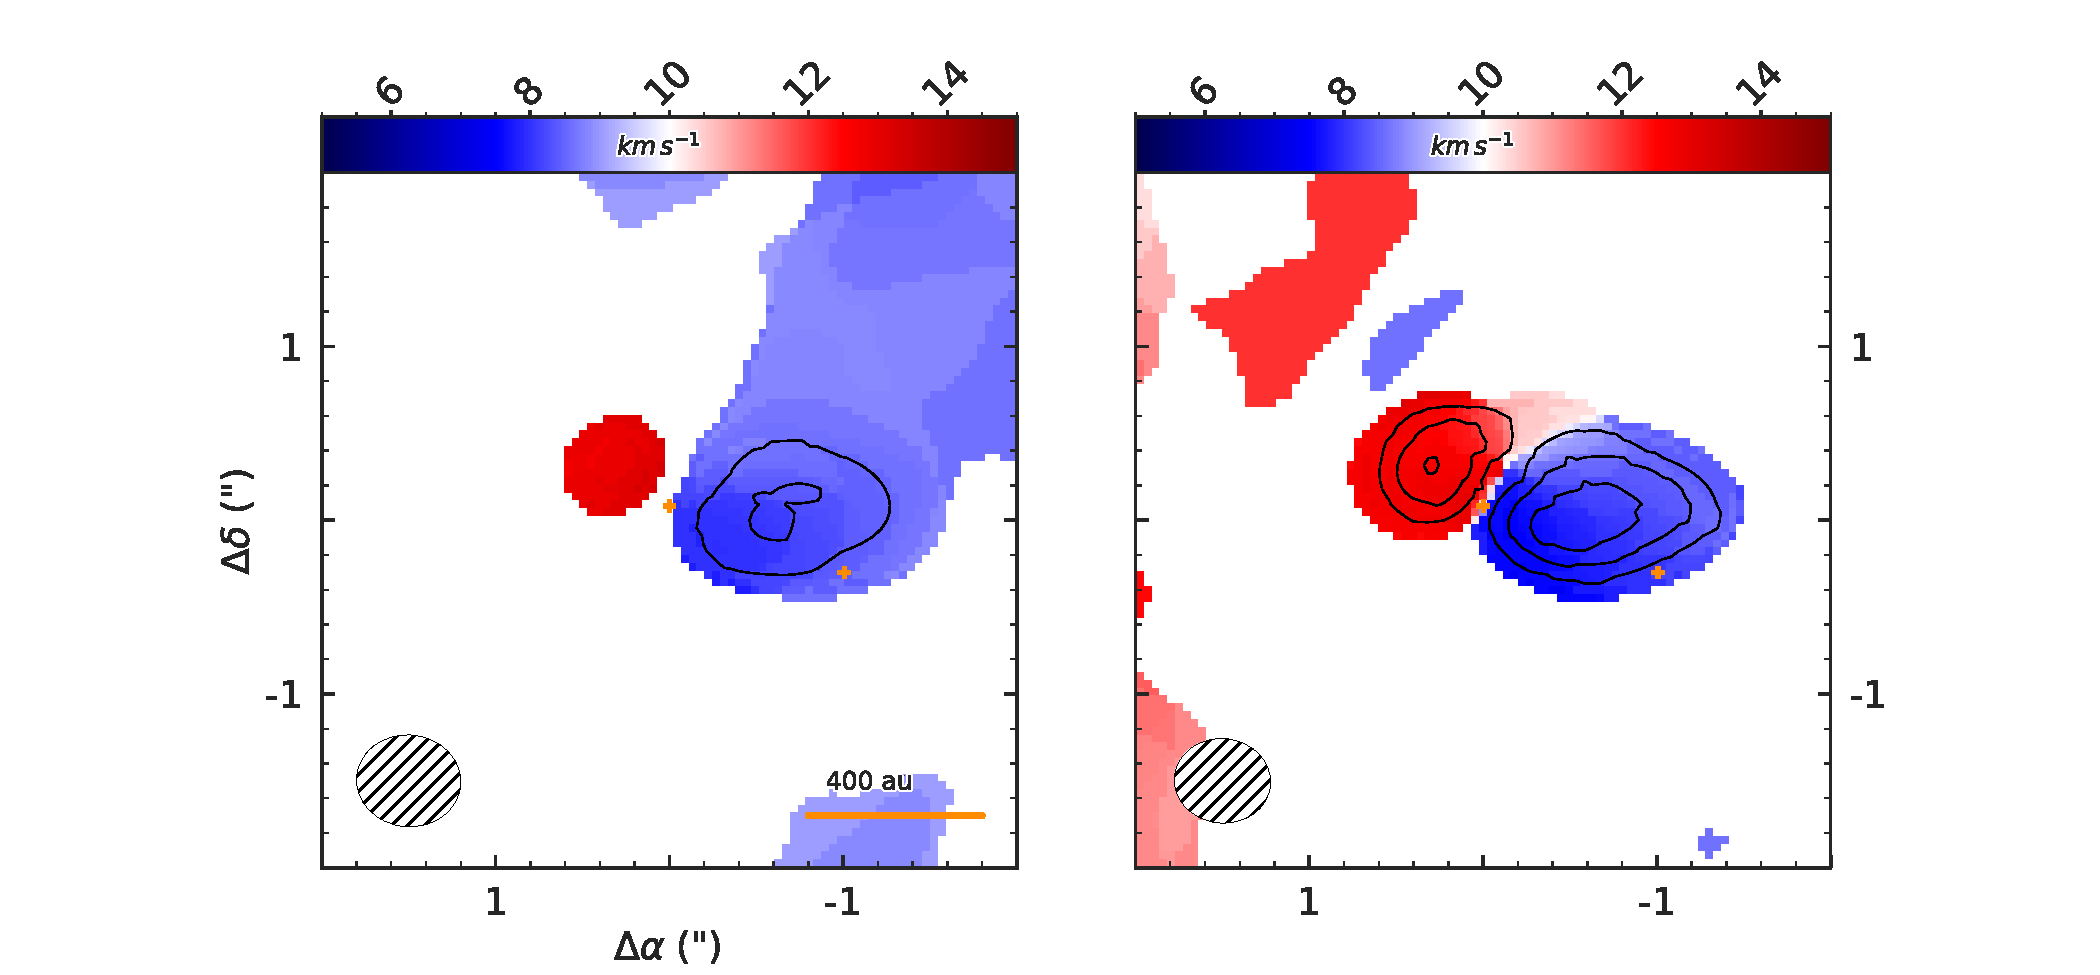
\includegraphics[width=.99\linewidth]{m1-map_co-co.pdf}
  \captionof{figure}{First moment map of HCN, with and without (below and above, respectively) baseline cuts.}
  \label{fig:test2}
\end{minipage}
\end{figure}
\fi



% Note that no closing info is needed.
